\section{Fourieroptik}
\subsection{Versuchsbeschreibung}

In diesem letzten Versuchsteil soll die Kreuzkorrelation und Faltung eines drehbaren Spaltes beobachtet werden. Dazu wird zunächst ein Hologramm der Fouriertransformierten dieses Spaltes erstellt. Nach der Entwicklung wird dieses dann ähnlich der Echtzeitspektroskopie mit der Fouriertransformierten des selben Spalts in verdrehter Einstellung überlagert. Je nach Betrachtungswinkel kann nun hinter der Platte entweder die die Faltung der beiden Apperturfunktionen (Spalte) oder deren Kreuzkorrelation betrachtet werden.

\begin{figure}[H]
 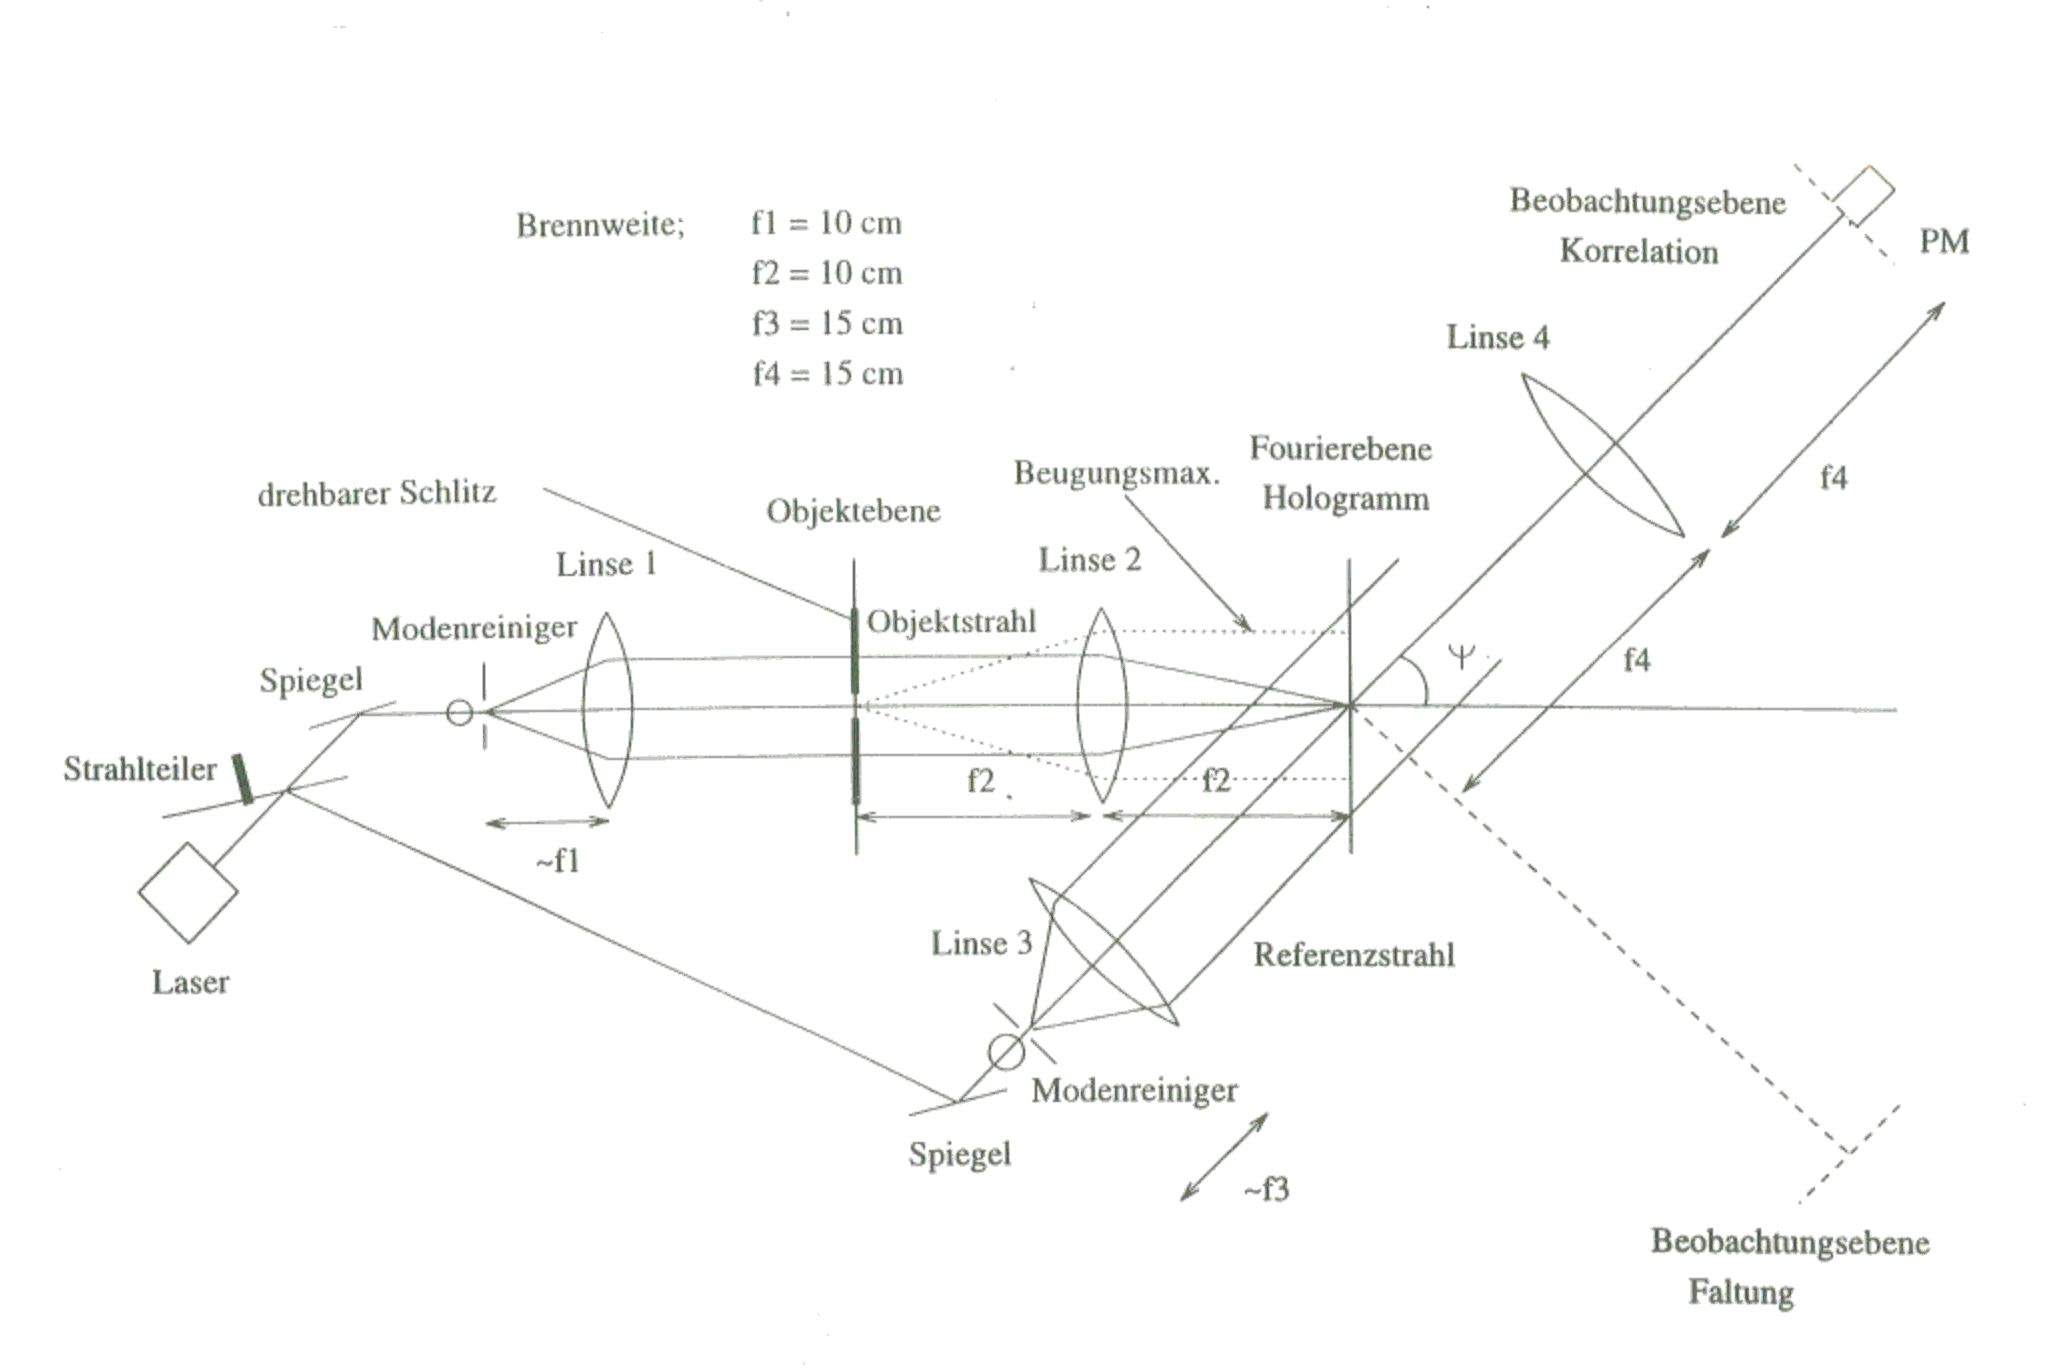
\includegraphics[width=\textwidth]{BilderAufbau/A-Bamberger-aufbau.png}
 \caption{Schematischer Versuchsaufbau für die Fourieroptik \cite{fourier}}
 \label{fourier_aufbau}
\end{figure}


\subsection{Durchführung und Auswertung}

Wir haben den Versuch wie in der Anleitung \cite{fourier} angegeben aufgebaut und ein Hologramm des Spaltes erstellt. Wir haben dabei die selben Parameter wie bei der Echtzeitholografie verwendet, die Belichtungszeit jedoch auf 3 min reduziert. Da bei diesem Aufbau mit dem direkten Strahl gearbeitet wird, ist die Intensität höher. Nach der Entwicklung waren sowohl das Hologramm des Spaltes als auch das Objektbild überlagert mit der Lupe zu sehen. Es war jedoch keine Wechselwirkung der beiden auszumachen, die zu einer Faltung oder Kreuzkorrelation geführt hätte.

\begin{figure}[H]
 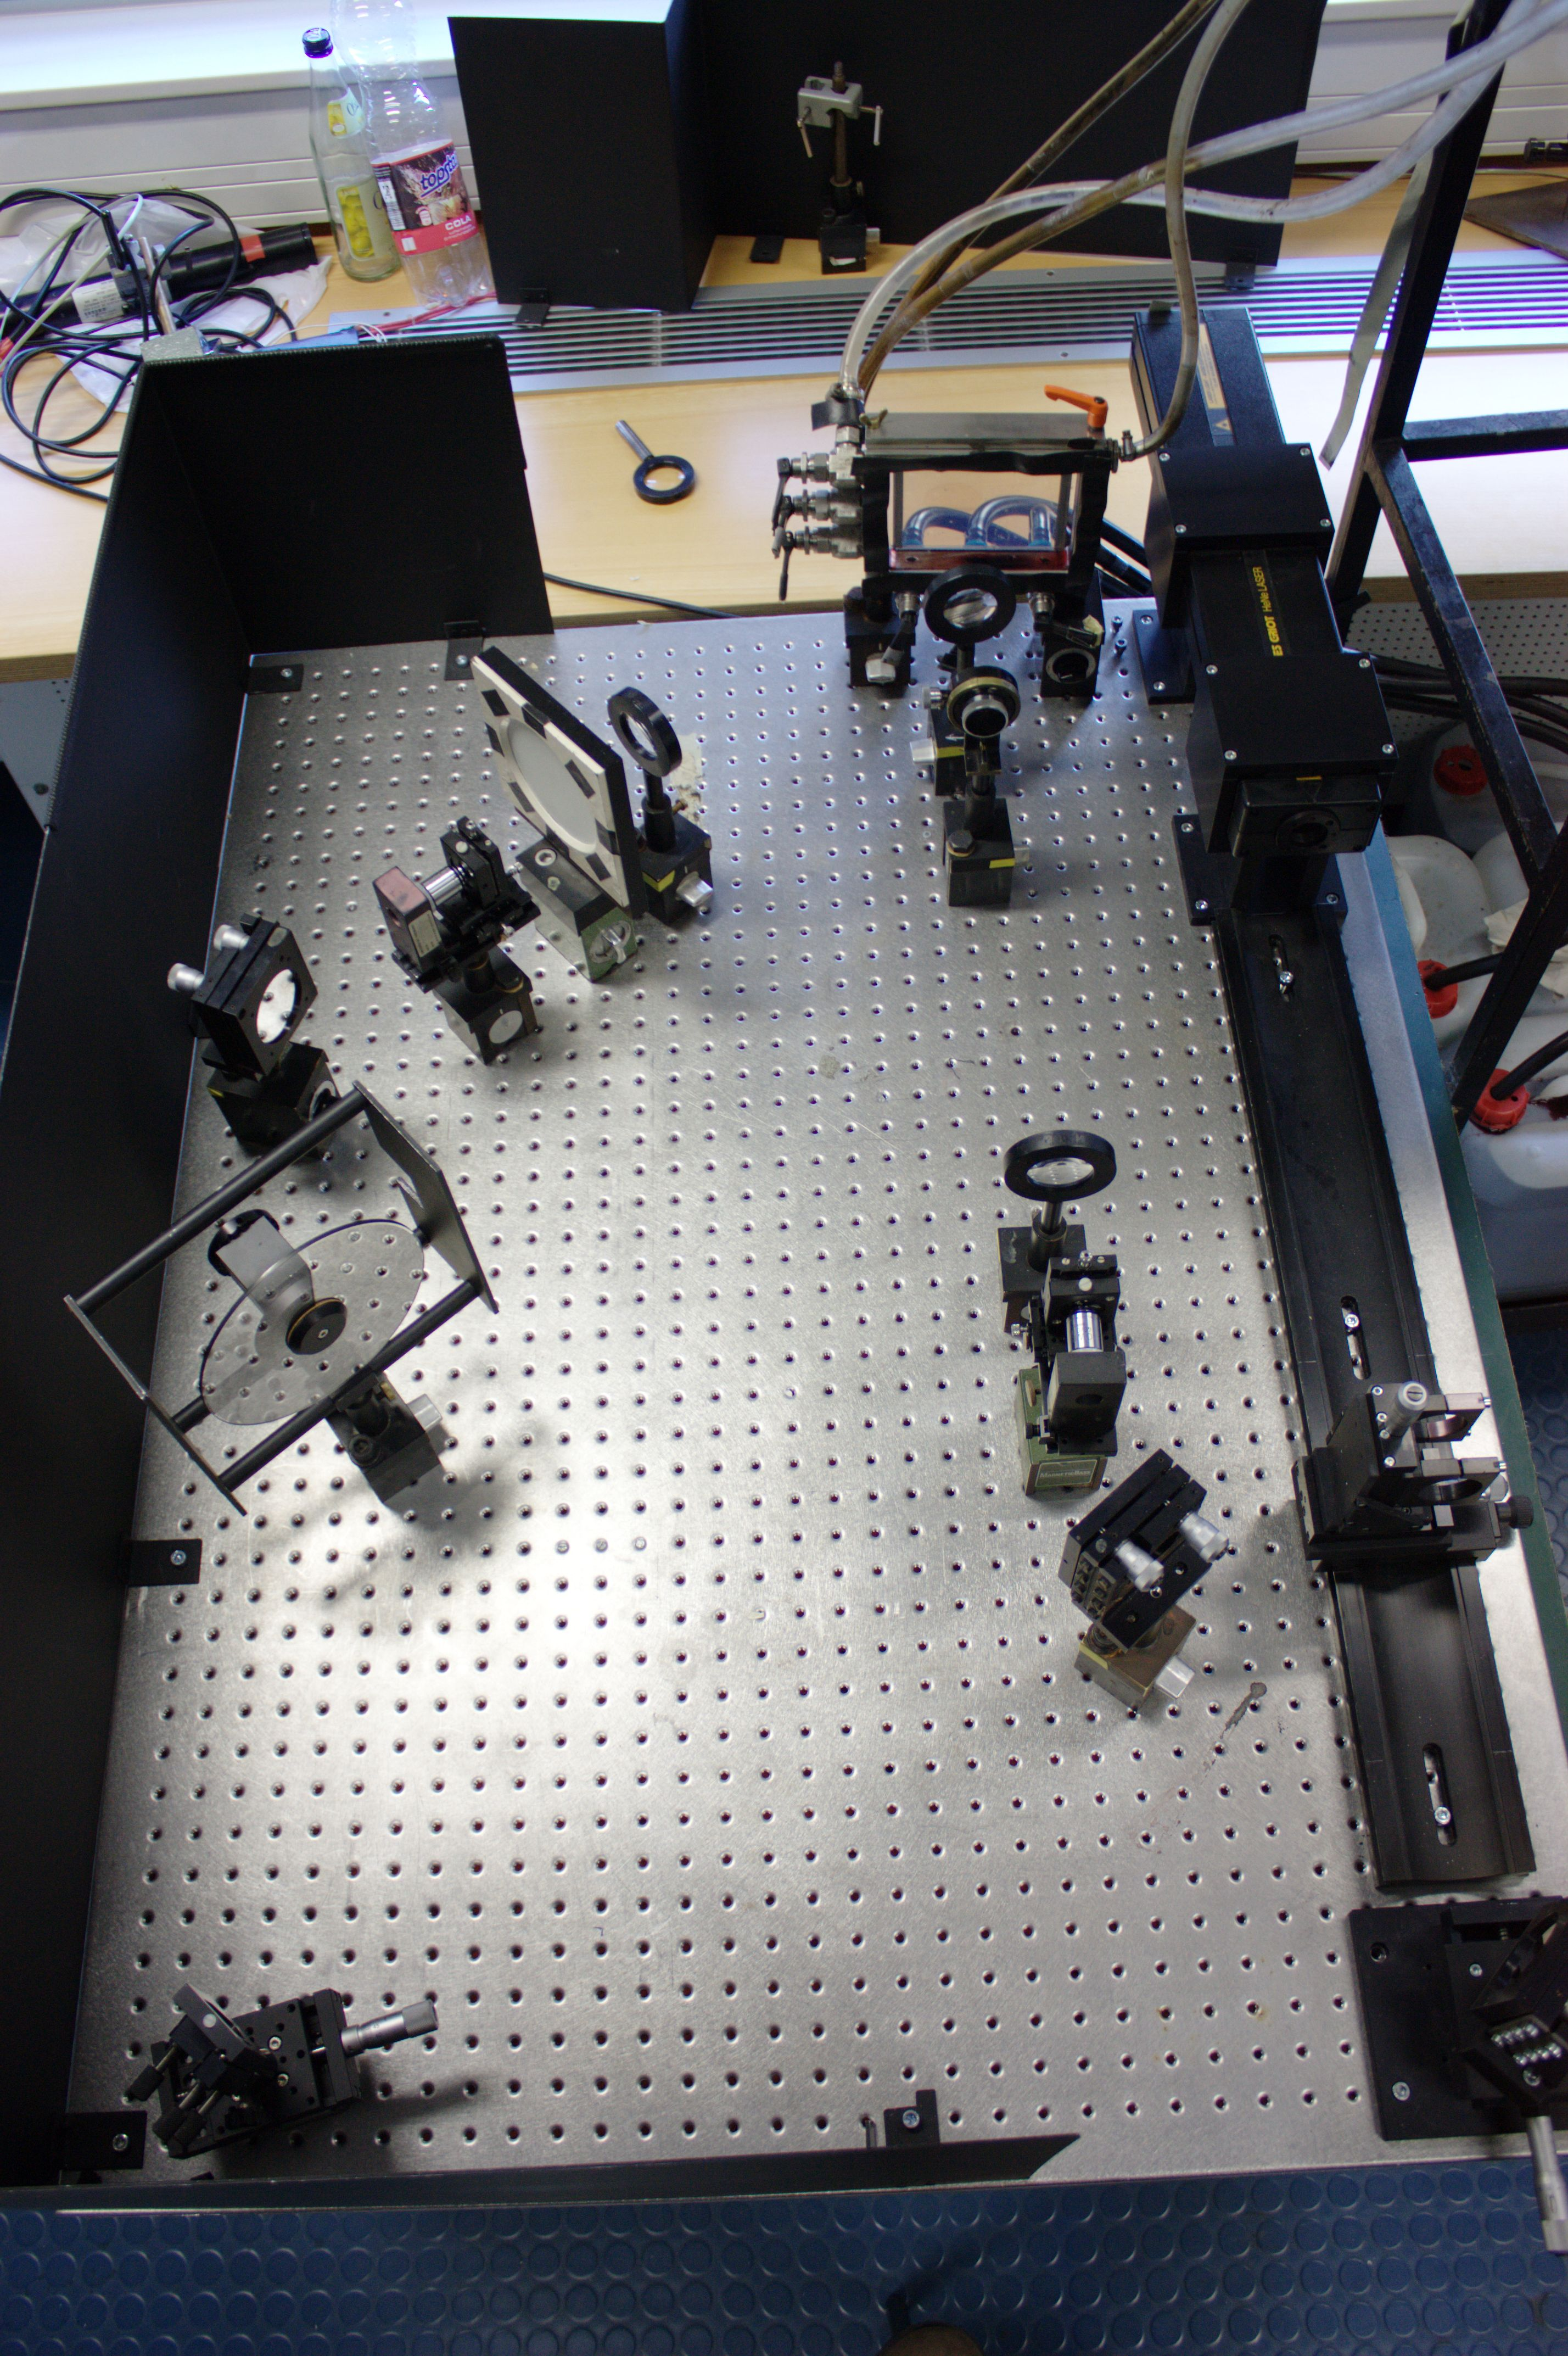
\includegraphics[height=0.5\textheight]{Photos/IMG_3941.jpg}
 \caption{Versuchsaufbau für die Fourieroptik}
 \label{fourier_bild}
\end{figure}

Als Ursache für das Fehlen der Faltung und Kreuzkorrelation gibt es eine Vielzahl an Möglichkeiten. Dies fängt damit an, dass wir uns zum Beobachten auf das Fensterbrett legen mussten und sowohl Lupe als auch Augen freihändig in die richtige Position bringen mussten. Ein längerer Versuchstisch hätte hier vielleicht Abhilfe geschaffen, wir waren jedoch bereits froh überhaupt einen schwingungsgedämpften zur Verfügung zu haben. Wenn dieses Problem (zufällig) einmal überwunden ist, bereiten natürlich immernoch eventuelle Verrückungen am Aufbau während der Aufnahme Probleme. Weiterhin könnte es sein, das wir die Fourierebene nicht korrekt mit der Hologrammebene in Einklang gebracht haben.
Da wir auch die Winkel zwischen Objektstrahl und Referenzstrahl sowie die Position der Platte ungünstig gewählt hatten, haben wir den Aufbau entsprechend angepasst (Abb \ref{fourier_bild}). Leider haben wir nicht ausreichend Entwicklerflüssigkeit in das Becken laufen lassen, so das nur die Hälfte des Bildes entwickelt wurde. Natürlich viel uns dies erst nach dem Bleichen auf. Somit war jetzt auch die verdünnte Bleiche auf eine minimale Restmenge zusammengeschrumpft und eine weitere Streckung mit Wasser (dann ca. 50:1) erschien uns fragwürdig. Eine weitergehende Optimierung der Parameter wie Spaltöffnung, Winkel, Strahlengang, Belichtungszeit etc. war uns deshalb leider nicht mehr möglich.